\documentclass{article}\usepackage[]{graphicx}\usepackage[]{xcolor}
% maxwidth is the original width if it is less than linewidth
% otherwise use linewidth (to make sure the graphics do not exceed the margin)
\makeatletter
\def\maxwidth{ %
  \ifdim\Gin@nat@width>\linewidth
    \linewidth
  \else
    \Gin@nat@width
  \fi
}
\makeatother

\definecolor{fgcolor}{rgb}{0.345, 0.345, 0.345}
\newcommand{\hlnum}[1]{\textcolor[rgb]{0.686,0.059,0.569}{#1}}%
\newcommand{\hlstr}[1]{\textcolor[rgb]{0.192,0.494,0.8}{#1}}%
\newcommand{\hlcom}[1]{\textcolor[rgb]{0.678,0.584,0.686}{\textit{#1}}}%
\newcommand{\hlopt}[1]{\textcolor[rgb]{0,0,0}{#1}}%
\newcommand{\hlstd}[1]{\textcolor[rgb]{0.345,0.345,0.345}{#1}}%
\newcommand{\hlkwa}[1]{\textcolor[rgb]{0.161,0.373,0.58}{\textbf{#1}}}%
\newcommand{\hlkwb}[1]{\textcolor[rgb]{0.69,0.353,0.396}{#1}}%
\newcommand{\hlkwc}[1]{\textcolor[rgb]{0.333,0.667,0.333}{#1}}%
\newcommand{\hlkwd}[1]{\textcolor[rgb]{0.737,0.353,0.396}{\textbf{#1}}}%
\let\hlipl\hlkwb

\usepackage{framed}
\makeatletter
\newenvironment{kframe}{%
 \def\at@end@of@kframe{}%
 \ifinner\ifhmode%
  \def\at@end@of@kframe{\end{minipage}}%
  \begin{minipage}{\columnwidth}%
 \fi\fi%
 \def\FrameCommand##1{\hskip\@totalleftmargin \hskip-\fboxsep
 \colorbox{shadecolor}{##1}\hskip-\fboxsep
     % There is no \\@totalrightmargin, so:
     \hskip-\linewidth \hskip-\@totalleftmargin \hskip\columnwidth}%
 \MakeFramed {\advance\hsize-\width
   \@totalleftmargin\z@ \linewidth\hsize
   \@setminipage}}%
 {\par\unskip\endMakeFramed%
 \at@end@of@kframe}
\makeatother

\definecolor{shadecolor}{rgb}{.97, .97, .97}
\definecolor{messagecolor}{rgb}{0, 0, 0}
\definecolor{warningcolor}{rgb}{1, 0, 1}
\definecolor{errorcolor}{rgb}{1, 0, 0}
\newenvironment{knitrout}{}{} % an empty environment to be redefined in TeX

\usepackage{amsmath}
\usepackage{alltt}
\usepackage[utf8]{inputenc}
\usepackage{amsfonts}
\usepackage{tgpagella}
\usepackage{graphicx} % Required for inserting images
\usepackage{polski}
\renewcommand*{\figurename}{Rysunek}
\usepackage{nicefrac, xfrac}
\usepackage[margin=1in]{geometry}
\usepackage{hyperref}
\usepackage{xcolor}
\usepackage{amssymb}
\usepackage[bottom]{footmisc}
\usepackage{float}

\date{\now}
\IfFileExists{upquote.sty}{\usepackage{upquote}}{}
\begin{document}

\begin{titlepage}
\end{titlepage}
\begin{center}
 {\LARGE\bfseries Projekt\\}
 \vspace{0.5cm}
 {\Huge\bfseries \color{magenta} Pimp My Wheels\\}
 \vspace{0.5cm}
 {\LARGE\bfseries Bazy danych\\}
 {\Large Prowadzący kurs: dr Tomasz Stroiński\\}
 % ----------------------------------------------------------------
 \vspace{1cm}
 {\Large\bfseries Autorzy:\\[4pt]}
 \vspace{1.5cm}
  {\Large\bfseries Weronika Kuzara\\[3pt]}
  \vspace{0.5cm}
 
 {\Large\bfseries Martyna Maciaszek\\[3pt]}
 \vspace{0.5cm}
 
 {\Large\bfseries Aleksander Rzyhak\\[3pt]}
 \vspace{0.5cm}
 
 {\Large\bfseries Oskar Matysik\\[3pt]}
 \vspace{0.5cm}
 
 {\Large\bfseries Aleksandra Palka\\[5pt]}
  % ----------------------------------------------------------------

 \vfill
{\Large \today}
\end{center}
\newpage



\section{Wstęp}
Raport jest przedostatnią częścią projektu polagającego na stworzeniu bazy danych warsztatu „Pimp My Wheels”. Został zaprojektowany schemat bazy danych, na podstawie którego została stworzona już właściwa baza. Następnie została ona wypełniona losowymi danymi.

Raport ma na celu przeanalizowanie działalności warsztatu „Pimp My Wheels” znajdującego się we Wrocławiu. Na moment, dla którego pisany był raport, warsztat działa od początku 2014 roku do końca 2017 roku. Firma zajmuje się prowadzeniem klasycznego warsztatu oraz skupem, renowacją i sprzedażą samochodów i motocykli. 

\section{Odsetek naprawianych marek pojazdów}
%Odsetek naprawianych marek pojazdów.

Przeprowadzono analizę, aby sprawdzić jakich marek pojazdy najczęściej pojawiają się w warsztacie do naprawy. 



Można przedstawić procentowy udział marek pojazdów klientów salonu, zaczynając od najczęściej się pojawiającej:

\begin{verbatim}
1. Volkswagen: 12,34%
2. Ford: 10,25%
3. Opel: 9,41%
4. Skoda: 6,49%
5. Audi: 5,86%
6. BMW: 5,23%
7. SEAT: 4,6%
8. Mercedes-Benz: 4,18%
9. Renault: 3,77%
10. Toyota: 3,14%
11. Hyundai: 2,93%
12. Peugeot: 2,93%
13. Hero: 2,72%
14. Honda: 2,51%
15. Fiat: 2,51%
16. Bajaj: 2,3%
17. Nissan: 2,09%
18. Mazda: 2,09%
19. Citroen: 1,88%
20. Volvo: 1,46%
21. Kia: 1,46%
22. smart: 1,26%
23. TVS: 1,05%
24. Royal: 1,05%
25. Suzuki: 1,05%
26. Yamaha: 0,63%
27. Mitsubishi: 0,63%
28. Dacia: 0,63%
29. Jeep: 0,63%
30. KTM: 0,42%
31. Subaru: 0,42%
32. Porsche: 0,42%
33. Estrima: 0,42%
34. MINI: 0,42%
35. Mahindra: 0,21%
36. Alfa: 0,21%
37. Chevrolet: 0,21%
38. McLaren: 0,21%
\end{verbatim}

Jak widać, najpopularniejsze są pojazdy marki Volkswagen. Pojazdy tej marki stanowią \text{12,34}\% wszystkich. \\

Najmniej popularne są marki Alfa, Chevrolet, McLaren i Mahindra. Każdą z nich reprezentowało 0,21\% pojazdów, które się pojawiły w warsztacie. Ilość pojazdów, które były w warsztacie to \text{478}. Było więcej samochodów niż motorów. Różnica między ilością obu typów pojazdu wynosiła \text{376}, a samochodów było \text{427}.

Sprawdzono także, jak prezentowałyby się rozkład marek, gdyby brano pod uwagę jedynie samochody



Można przedstawić ranking marek, zaczynając od najczęściej się pojawiającej:

\begin{verbatim}
1. Volkswagen: 13,82%
2. Ford: 11,48%
3. Opel: 10,54%
4. Skoda: 7,26%
5. Audi: 6,56%
6. BMW: 5,85%
7. SEAT: 5,15%
8. Mercedes-Benz: 4,68%
9. Renault: 4,22%
10. Toyota: 3,51%
11. Hyundai: 3,28%
12. Peugeot: 3,28%
13. Fiat: 2,81%
14. Mazda: 2,34%
15. Nissan: 2,34%
16. Citroen: 2,11%
17. Kia: 1,64%
18. Volvo: 1,64%
19. smart: 1,41%
20. Suzuki: 1,17%
21. Mitsubishi: 0,7%
22. Jeep: 0,7%
23. Dacia: 0,7%
24. Subaru: 0,47%
25. Porsche: 0,47%
26. Estrima: 0,47%
27. MINI: 0,47%
28. Honda: 0,23%
29. Alfa: 0,23%
30. Chevrolet: 0,23%
31. McLaren: 0,23%
\end{verbatim}

Wśród aut prym wiedzie Volkswagen, reprezentując  13,82\% naprawianych samochodów. Najmniej było samochodów marek Alfa, Chevrolet, McLaren i Honda. Było ich 0,23\% dla każdej. \\

Pozostały do sprawdzenia motory.



Udział procentowy poszczególnych marek wśród nich prezentuje się następująco:

\begin{verbatim}
1. Hero: 25,49%
2. Bajaj: 21,57%
3. Honda: 21,57%
4. Royal: 9,8%
5. TVS: 9,8%
6. Yamaha: 5,88%
7. KTM: 3,92%
8. Mahindra: 1,96%
\end{verbatim}

Wśród nich najczęściej naprawiano motory marki Hero. Pojazdy tej marki stanowią 25,49\% wszystkich. Najmniej popularnymi motorami są z kolei modele marki Mahindra. W warsztacie było zaledwie 1,96\% motorów tej marki.

\section{Liczba naprawianych pojazdów w każdym miesiącu pracy warsztatu}

\begin{knitrout}
\definecolor{shadecolor}{rgb}{0.969, 0.969, 0.969}\color{fgcolor}\begin{figure}[H]

{\centering 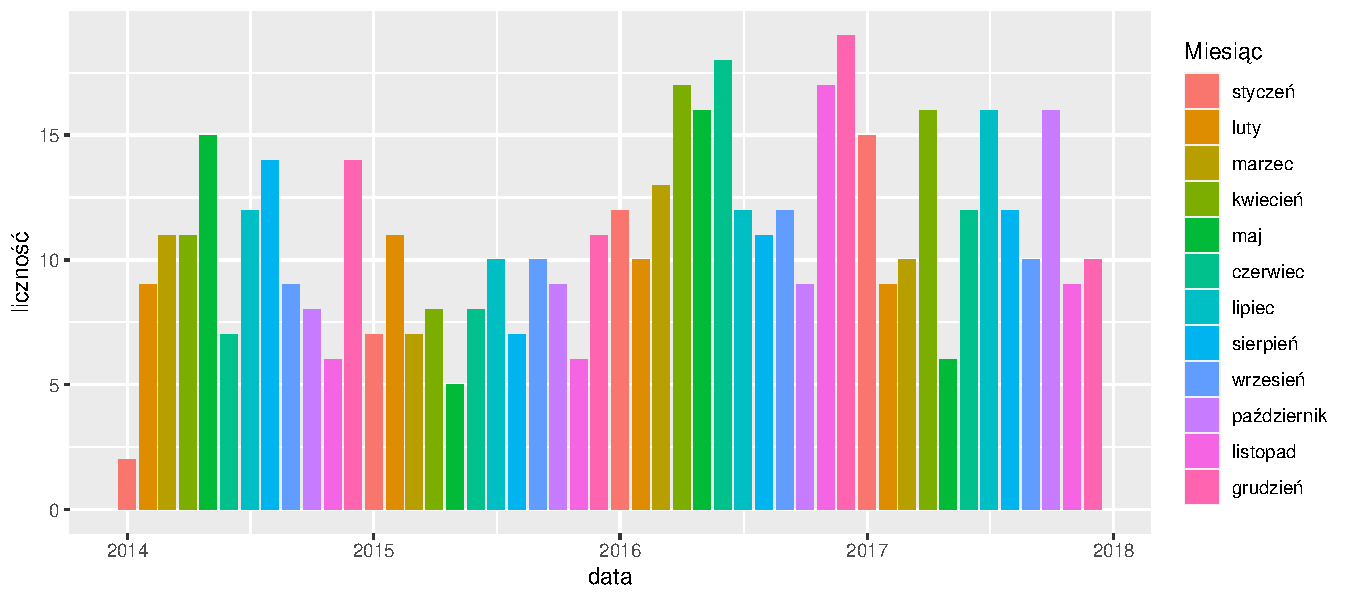
\includegraphics[width=\maxwidth]{figure/fig_naprawy_miesiecznie-1} 

}

\caption[Wykres liczba naprawianych pojazdów w każdym miesiącu pracy warsztatu]{Wykres liczba naprawianych pojazdów w każdym miesiącu pracy warsztatu}\label{fig:fig_naprawy_miesiecznie}
\end{figure}

\end{knitrout}

Wykres \ref{fig:fig_naprawy_miesiecznie} przedstawia liczbę naprawionych pojazdów w każdym miesiącu pracy warsztatu. Najwięcej pojazdów zostało naprawionych w miesiącu 
grudzień 2016,
a było ich \text{18}. Natomiast najmniej przeprowadzonych napraw było w miesiącu
styczeń 2014,
było ich \text{0}. Średnia liczba napraw miesięcznie wynosi 
\text{9,96}. 

\section{Tabela najlepszych okazji}

Zostanie teraz omówiona tabela najlepszych okazji, czyli pojazdów skupionych i sprzedanych, które przyniosły najwięcej zysku. Został uwzględniony także koszt naprawy pojazdu, gdy była ona potrzebna.





\begin{knitrout}
\definecolor{shadecolor}{rgb}{0.969, 0.969, 0.969}\color{fgcolor}\begin{kframe}
\begin{verbatim}
##     id_samochodu   marka model   zysk
## 278          366  Alpina    B5 168512
## 150          181   Mazda  CX-5  95402
## 571          181   Mazda  CX-5  93600
## 470          601 Porsche Macan  78542
## 609          768   Volvo  XC60  76178
\end{verbatim}
\end{kframe}
\end{knitrout}

Największy zysk ze sprzedaży pojazdu warsztat odniósł dla pojazdu o id \text{366}. Jest nim Alpina o modelu B5. Warsztat zarobił on na nim około 168,51 tyś. zł. 
Na drugim miejscu znajduje się Mazda o modelu CX-5. Zysk z tego pojazdu wyniósł około 95,4 tyś. zł, czyli o około 73,11 tyś. zł mniej niż dla pojazdu znajdującego się na pierwszym miejscu, czyli różnica w cenie jest duża.
W trzeciej kolejności najwięcej zarobił pojazd Mazda o modelu CX-5, na którym warsztat zarobił około 93,6 tyś. zł. Jest to mniej od poprzedniego pojazdu o około 1,8 tyś. zł, czyli różnica w cenie jest duża. 
Ogólnie każdy pojazd znajdujący się w top 5 najlepszych okazji przyniósł zysk wielkości przynajmnej 80 tyś. zł.

\section{Profil klienta}

W następnej kolejności zostaną przeanalizawani klienci warsztatu. Zostaną sprawdzone liczności klientów ze względu na różne ich cechy.

\subsection{Płeć}

Pierwszą cechą wziętą pod uwagę jest płeć klienta. Zostanie sprawdzone, ile jest kobiet i mężczyzn wśród naszych klientów oraz jak duża jest różnica w licznościach tych grup.

\begin{knitrout}
\definecolor{shadecolor}{rgb}{0.969, 0.969, 0.969}\color{fgcolor}\begin{figure}[H]

{\centering 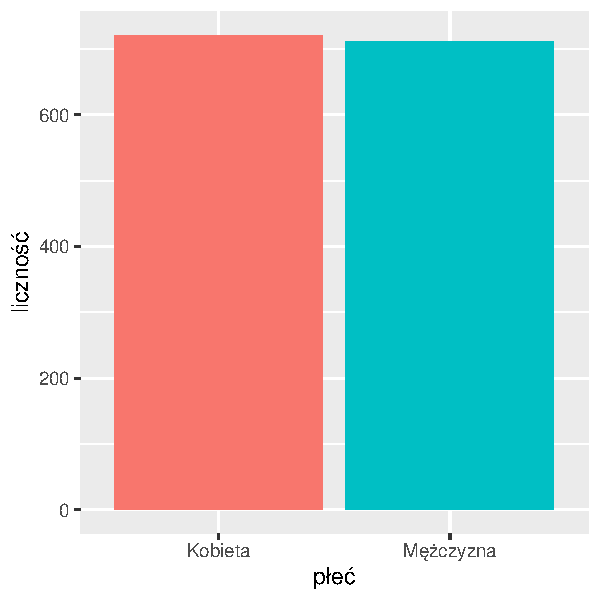
\includegraphics[width=\maxwidth]{figure/fig_plec-1} 

}

\caption[Wykres liczby klientów przy podziale ze względu na płeć]{Wykres liczby klientów przy podziale ze względu na płeć}\label{fig:fig_plec}
\end{figure}

\end{knitrout}

Na wykresie słupkowym \ref{fig:fig_plec} są zaprezentowane liczności klientów przy podziale ze względu na płeć. Więcej klientów warsztatu należy do grupy kobiet, jest ich \text{699}. Grupa kobiet jest około \text{1,015}
razy większa od grupy mężczyzn (jest ich \text{689}), a zatem różnica jest nieduża.

\subsection{Wiek}

Zostanie również przeanalizowany rozkład wieku klientów warsztatu.





\begin{knitrout}
\definecolor{shadecolor}{rgb}{0.969, 0.969, 0.969}\color{fgcolor}\begin{figure}[H]

{\centering 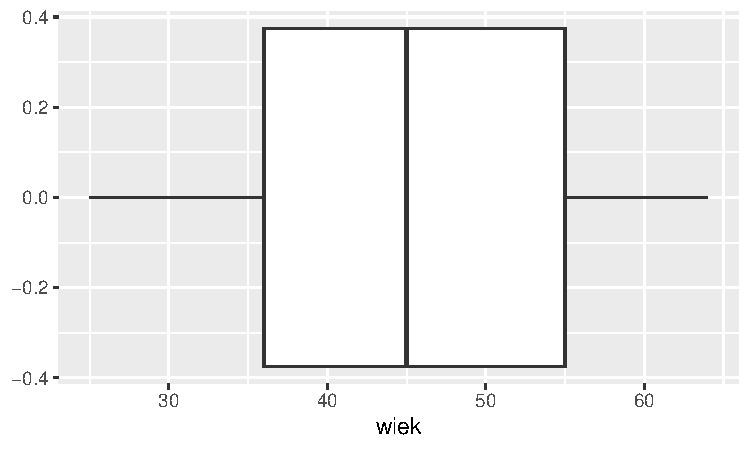
\includegraphics[width=\maxwidth]{figure/fig_wiek-1} 

}

\caption[Wykres pudełkowy wieku klientów]{Wykres pudełkowy wieku klientów}\label{fig:fig_wiek}
\end{figure}

\end{knitrout}

Rysunek \ref{fig:fig_wiek} przedstawia wykres pudełkowy wieku klientów warsztatu. Widać, że mediana wieku wynosi \text{45} lat, natomiast pierwszy kwartyl wynosi \text{36} lat, a trzeci kwartyl \text{54} lata. Zatem połowa klientów warsztatu jest wieku między \text{36} lat a \text{54} lata.
Najmłodszy klient warsztatu ma \text{25} lat, natomiast najstarszy jest w wieku \text{64} lat.



\begin{table}[H]
\centering
\begin{tabular}{c|c} \hline
Miara & Wartość \\ \hline
Średnia & \text{44,9} \\ 
Odchylenie standardowe & \text{10,61} \\
Skośność & \text{0,02}  \\ 
Kurtoza & \text{1,88} \\ \hline
\end{tabular}
\caption{Wybrane miary wieku klientów}
\label{tab_wiek}
\end{table}

Kilka miar, których nie da się odczytać z wykresu pudełkowego, zostało przedstawionych w tabeli \ref{tab_wiek}. Można zatem odczytać, że średnio klieci mają \text{44,9} lat, a odchylenie standardowe wieku wynosi \text{10,61} lat. Wartość współczynnika skośności jest bliska 0, a zatem rozkład wieku można uznać za symetryczny. Kurtoza przyjmuje wartość większą od 0, a zatem rozkład wieku jest leptokurtyczny, czyli jest bardziej wysmukły niż normalny.

\subsection{Miasto}
\begin{knitrout}
\definecolor{shadecolor}{rgb}{0.969, 0.969, 0.969}\color{fgcolor}\begin{kframe}
\begin{verbatim}
##   miejsce              miasto liczność
## 1     1,0             Wrocław      735
## 2     2,0            Warszawa       19
## 3     3,5                Łódź       18
## 4     3,5               Opole       18
## 5     5,5 Gorzów Wielkopolski       16
## 6     5,5              Poznań       16
\end{verbatim}
\end{kframe}
\end{knitrout}

Najwięcej klientów warsztatu pochodzi z miasta Wrocław. Liczniść w nim wynosi \text{735} klientów. W następnej kolejności najwięcej klientów pochodzi z miasta Warszawa, z czego liczność w nim wynosi \text{19} klientów, czyli jest ich \text{38,68} mniej niż klientów z miasta Wrocław. Na miejscu \text{3,5} są miasta Łódź, Opole, mieszka w nich \text{18} klientów. Natomiast na ostatnim miejscu przedstawionym w tabeli są miasta Gorzów Wielkopolski, Poznań, mieszka w nich \text{16} klientów.

\subsection{Karta lojalnościowa}

W tej części zostanie sprawdzone ilu klientów posiada kartę lojalnościową. Klient zdobywa ją po skorzystaniu z usług warsztatu (naprawa, zakup lub sprzedaż pojazdu) przynajmniej trzy razy. Klient posiadający tę kartę może kupować samochody ze zniżką w wysokości 3\%.

\begin{knitrout}
\definecolor{shadecolor}{rgb}{0.969, 0.969, 0.969}\color{fgcolor}\begin{figure}[H]

{\centering 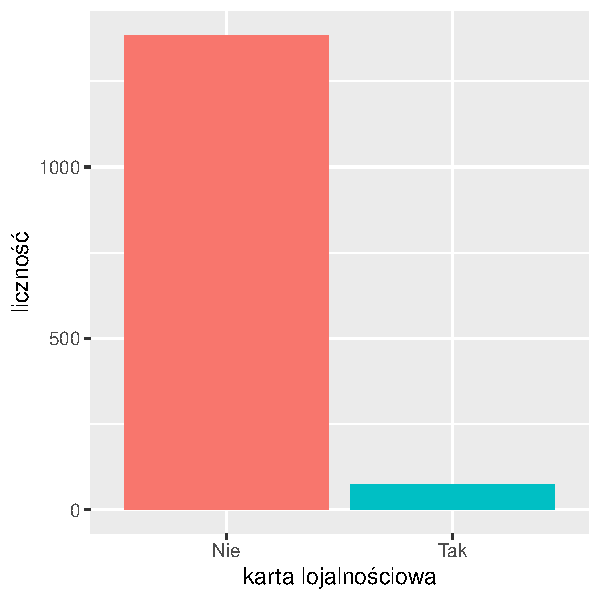
\includegraphics[width=\maxwidth]{figure/fig_karta-1} 

}

\caption[Wykres liczby klientów ze względu na posiadanie karty lojalnościowej]{Wykres liczby klientów ze względu na posiadanie karty lojalnościowej}\label{fig:fig_karta}
\end{figure}

\end{knitrout}

Bardziej liczną grupą są klienci, którzy nie posiadają karty lojalnościowej, jest ich \text{1311} (\text{94}\% wszystkich klientów). W grupie klientów, którzy posiadają kartę lojalnościową, jest \text{77} osób i stanowią oni \text{6}\% klientów warsztatu.

\section{Jak wybrane cechy pojazdów wpływają na zysk warsztatu?}

W tym paragrafie zostaną opisane zależności między zyskiem ze sprzedaży pojazdów, skupionych i w razie potrzeby naprawionych przez warsztat, a cechami: rodzaj pojazdu, czy jest powypadkowy i pojemność silnika.

\subsection{Rodzaj pojazdu}

Pierwszą cechą braną pod uwagę jest rodzaj pojazdu, czyli czy jest to samochód czy motocykl.

\begin{knitrout}
\definecolor{shadecolor}{rgb}{0.969, 0.969, 0.969}\color{fgcolor}\begin{figure}[H]

{\centering 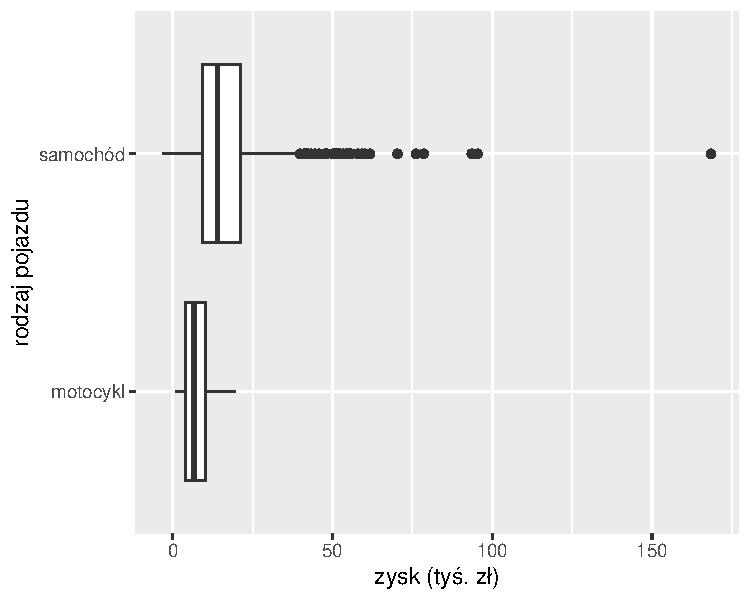
\includegraphics[width=\maxwidth]{figure/fig_typ-1} 

}

\caption[Wykresy pudełkowe zysku ze względu na rodzaj pojazdu]{Wykresy pudełkowe zysku ze względu na rodzaj pojazdu}\label{fig:fig_typ}
\end{figure}

\end{knitrout}

Na rysunku \ref{fig:fig_typ} przedstawione są dwa wykresy pudełkowe zysków, jeden dla samochodów, drugi dla motocykli. Większa mediana, wynosząca 13,98 tyś. zł, jest dla pojazdów typu samochód. W drugiej grupie wynosi ona 6,6 tyś. zł. 
Większy pierwszy kwartyl występuje w grupie typu samochód, wynosi on 9,21 tyś. zł, w porównaniu dla grupy typu motocykl jego wartość wynosi 3,95 tyś. zł.
W przypadku kwartyla trzeciego większa wartość występuje w grupie typu samochód (wynosi 21,31 tyś. zł). W drugiej grupie wynosi on 10,24 tyś. zł.
Największy zysk przyniósł samochód, a wyniósł on 168,51 tyś. zł. 
Najmniejszy zysk natomiast przyniósł samochód i wyniósł on -3,1 tyś. zł. Zatem częściej większy zysk dla warsztatu przynosi sprzedaż pojazdów typu samochód. 

\subsection{Czy powypadkowy}

Następną badaną cechą jest to, czy pojazd jest powypadkowy.

\begin{knitrout}
\definecolor{shadecolor}{rgb}{0.969, 0.969, 0.969}\color{fgcolor}\begin{figure}[H]

{\centering 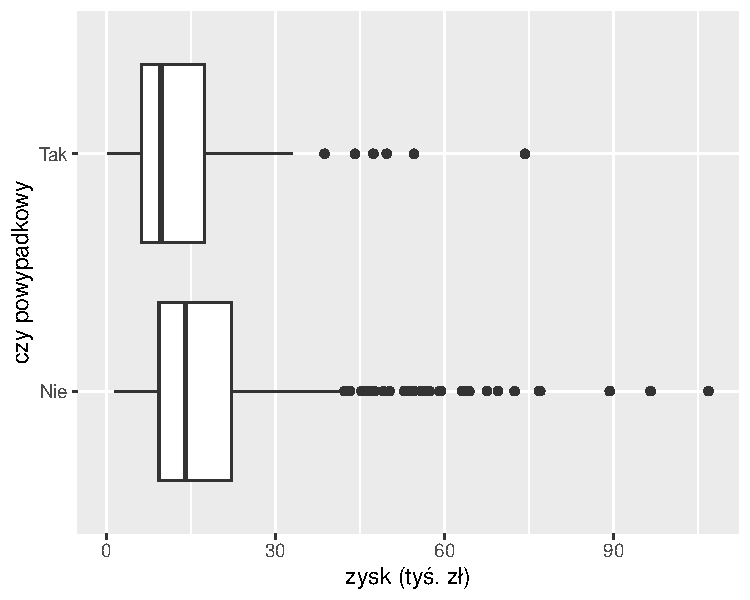
\includegraphics[width=\maxwidth]{figure/fig_wypadkowy-1} 

}

\caption[Wykresy pudełkowe zysku ze względu na to czy pojazd jest powypadkowy]{Wykresy pudełkowe zysku ze względu na to czy pojazd jest powypadkowy}\label{fig:fig_wypadkowy}
\end{figure}

\end{knitrout}

Na rysunku \ref{fig:fig_wypadkowy} przedstawione są dwa wykresy pudełkowe zysków dla pojazdów powypadkowych i niepowypadkowych. Większa mediana, wynosząca 13,78 tyś. zł, jest dla pojazdów niepowypadkowych. W drugiej grupie wynosi ona 10,1 tyś. zł. 
Większy pierwszy kwartyl występuje w grupie pojazdów niepowypadkowych, wynosi on 9,12 tyś. zł, w porównaniu dla grupy pojazdów powypadkowych jego wartość wynosi 6,65 tyś. zł.
Większa wartość trzeciego kwartylu występuje dla pojazdów niepowypadkowych i wynosi 20,86 tyś. zł. Dla pojazdów powypadkowych wynosi on 15,73 tyś. zł.
Największy zysk przyniósł pojazd z grupy niepowypadkowych i wyniósł on 168,51 tyś. zł. 
Najmniejszy zysk natomiast przyniósł pojazd z grupy niepowypadkowych i wyniósł on -3,1 tyś. zł. Zatem częściej większy zysk dla warsztatu przynosi sprzedaż pojazdów niepowypadkowych. 

\subsection{Pojemność silnika}

Ostatnią cechą braną pod uwagę jest pojemność silnika pojazdu.

\begin{knitrout}
\definecolor{shadecolor}{rgb}{0.969, 0.969, 0.969}\color{fgcolor}\begin{figure}[H]

{\centering 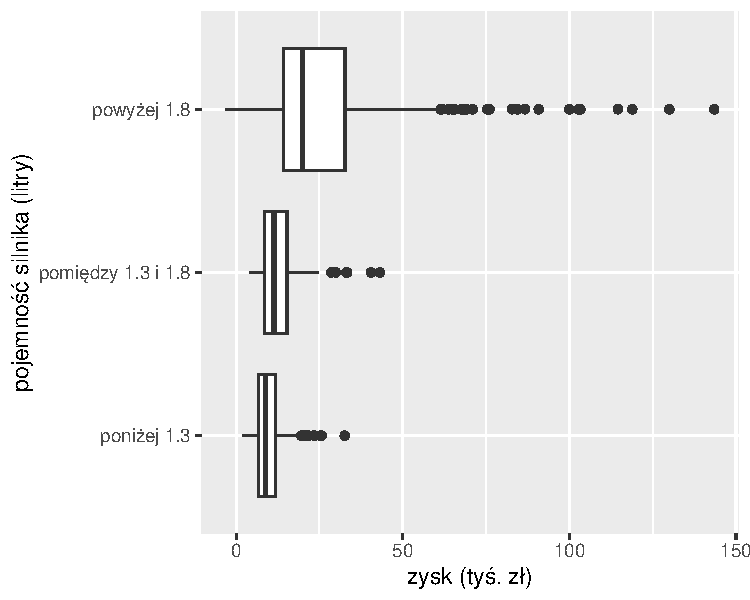
\includegraphics[width=\maxwidth]{figure/fig_pojemnosc-1} 

}

\caption[Wykresy pudełkowe zysku ze względu na pojemność silnika]{Wykresy pudełkowe zysku ze względu na pojemność silnika}\label{fig:fig_pojemnosc}
\end{figure}

\end{knitrout}

Na rysunku \ref{fig:fig_wypadkowy} przedstawione są wykresy pudełkowe zysków ze względu na pojemność silnika. Największa mediana, wynosząca 20,18 tyś. zł, jest dla pojazdów o pojemności silnika powyżej 1,8 litra. Natomiast najmniej ona wynosi 7,93 tyś. zł w grupie pojazdów o pojemności poniżej 1,3 litra. 
Największy pierwszy kwartyl występuje w grupie pojazdów o pojemności powyżej 1,8 litra, wynosi on 14,65 tyś. zł, w porównaniu z pojazdami o pojemności poniżej 1,3 litra, dla których jego wartość jest najmniejsza i wynosi 5,4 tyś. zł.
Największa wartość trzeciego kwartylu występuje dla pojazdów o pojemności powyżej 1,8 litra i wynosi 30,01 tyś. zł. Dla pojazdów poniżej 1,3 litra wynosi on 10,66 tyś. zł i jest to najmnijesza wartość w tych grupach.
Największy zysk przyniósł pojazd o pojemności silnika powyżej 1,8 litra i wyniósł on 168,51 tyś. zł. 
Najmniejszy zysk natomiast przyniósł pojazd z pojemnością silnika pomiędzy 1,3 i 1,8 litra i wyniósł on -3,1 tyś. zł. Zatem przeważnie największy zysk dla warsztatu przynosi sprzedaż pojazdów o pojemności silnika powyżej 1,8 litra. Najczęściej najmniejszy zysk przynosi sprzedaż pojazdów z pojemnością silnika poniżej 1,3 litra.

\section{Kim są najlepszy mechanik i sprzedawca w warsztacie?}

Przez czas działania warsztatu „Pimp My Wheels” osoba zarządzająca warsztatem nie była skłonna do dawania podwyżek, jednak postanowiła zlecić informatykowi by przeanalizował bazę danych i znalazł pracowników, którzy zasługują na większe wynagrodzenie. \\

Warsztatowi zależy na tym by sprzedawca zarobił dla firmy dużą kwotę (Może to osiągnąć sprzedając bardzo dużo pojazdów albo sprzedając wartościowe pojazdy), ale także by był charyzmatyczny i był w stanie przekonać wiele osób do zakupu. Rozważone wobec tego zostanie to który obecnie pracujący sprzedawca przekonał klientów do kupna największej liczby pojazdów, a który odpowiada za najwięcej środków pochodzących ze sprzedaży. \\


Tabela, w której są dane o sprzedawcach  pracujących w dowolnym momencie w warsztacie wygląda następująco:

\begin{knitrout}
\definecolor{shadecolor}{rgb}{0.969, 0.969, 0.969}\color{fgcolor}\begin{kframe}
\begin{verbatim}
##         sprzedawca     suma ile_sprzedanych płaca id_pracownika status
## 1  Sylwia Rakowska 21164080             363    46             3      0
## 2 Bogdan Kudrevych 21381016             367    50             2      1
\end{verbatim}
\end{kframe}
\end{knitrout}

Jeżeli pracownik odszedł z warsztatu, to nielogicznym jest, by rozważać danie mu podwyżki.

Po usunięciu pracowników, którzy już nie pracują otrzymujemy taką tabelę:

\begin{knitrout}
\definecolor{shadecolor}{rgb}{0.969, 0.969, 0.969}\color{fgcolor}\begin{kframe}
\begin{verbatim}
##         sprzedawca     suma ile_sprzedanych płaca id_pracownika status
## 1 Bogdan Kudrevych 21381016             367    50             2      1
\end{verbatim}
\end{kframe}
\end{knitrout}

Obecnie tylko jedna osoba pracuje w firmie na tym stanowisku i jest to Bogdan Kudrevych. Ta osoba sprzedała pojazdy łącznie na kwotę wynoszącą 21381015,96 zł na sprzedaży pojazdów, co stanowi 100,51\% średniej sumy całej kwoty, którą wynegocjował z klientami sprzedawca przez cały okres pracy. Zarabiana przez tego pracownika kwota za godzinę pracy (50,00 zł) stanowi 104,17 \% średniej płacy sprzedawcy (48,00 zł). Różnica procentowa wynosi 3,66\% na korzyść pracownika, jednak biorąc pod uwagę, że to jedyna osoba pracująca obecnie jako sprzedawca w warsztacie i była porównywana z byłymi pracownikami, można jej zaoferować podniesienie płacy, by pozytywnie wpłynąć na jej motywację. \\

Ten sprzedawca namówił klientów do kupna pojazdów w liczbie 367, co stanowi 100,55\% ilości sprzedanych pojazdów dzielonej przez liczbę kiedykolwiek zatrudnionych pracowników. Podobnie jak wcześniej, możemy spróbować porównać zarobki z ilością sprzedaży. różnica między stosunkiem zarobków do średniej płacy i sprzedanych przez obecnego sprzedawcę samochodów do średniej liczby przypadającej na sprzedawcę  wynosi 3,62\%. Gdyby jedynie brać pod uwagę ilość sprzedaży przy analizie to możnaby było zauważyć, że różnica jest na korzyść pracownika. Drobna podwyżka może jednak okazać się dla niego dobrym motywatorem. 

\begin{knitrout}
\definecolor{shadecolor}{rgb}{0.969, 0.969, 0.969}\color{fgcolor}\begin{kframe}
\begin{verbatim}
##              mechanik  suma ile_napraw płaca id_pracownika status
## 1   Wiktoria Kamińska 56286        121  48,9             6      0
## 2 Małgorzata Mrzygłód 68371        151  55,6             8      1
## 3       Lilla Kotynia 71598        153  53,8             9      1
## 4         Jane Chocyk 77660        121  50,2             7      1
## 5     Krystyna Konina 82081        152  57,5             4      1
\end{verbatim}
\end{kframe}
\end{knitrout}


Tutaj również należy usunąć z tabeli mechaników, którzy już nie pracują w warsztacie. \\

Pozostali następujący pracownicy:

\begin{knitrout}
\definecolor{shadecolor}{rgb}{0.969, 0.969, 0.969}\color{fgcolor}\begin{kframe}
\begin{verbatim}
##              mechanik  suma ile_napraw płaca id_pracownika status
## 1 Małgorzata Mrzygłód 68371        151  55,6             8      1
## 2       Lilla Kotynia 71598        153  53,8             9      1
## 3         Jane Chocyk 77660        121  50,2             7      1
## 4     Krystyna Konina 82081        152  57,5             4      1
\end{verbatim}
\end{kframe}
\end{knitrout}

Mechanik, który wykonał w firmie naprawy, za które klienci (po odliczeniu kosztu części) zapłacili najwięcej to Krystyna Konina i jest to kwota 82081,00 zł, co stanowi 115,28\% średniego zysku z napraw na mechanika. Pracownik zarabia kwotę 57,50 zł za godzinę pracy, co stanowi 108,08 \% średniej płacy mechanika (53,20 zł). Różnica między tymi wartościami to 7,20\%, wobec czego dobrze by było, gdyby firma zauważyła świetne wyniki tego pracownika i jego pozytywny wpływ na finanse warsztatu. \\

Pracownik, który dokonał największej liczby napraw to Lilla Kotynia. Liczba napraw dokonana przez niego wynosi 153, co stanowi 110,07\% średniej ilości napraw na mechanika. Jej zarobki wynoszą 53,80 zł na godzinę, co stanowi 101,13 \% średniej płacy mechanika (53,20 zł). Różnica między tymi dwoma wartościami wynosi 8,94\%, więc podwyżka wydaje się rozsądnym rozwiązaniem, aby okazać mechanikowi, że warsztat go docenia.

\section{Analiza bilansu}

\subsection{Analiza wydatków na zakup pojazdów}

Sprawdziliśmy, jak wyglądają miesięczne wydatki na zakup pojazdów, które w razie potrzeby warsztat naprawia, a następnie sprzedaje.

\begin{knitrout}
\definecolor{shadecolor}{rgb}{0.969, 0.969, 0.969}\color{fgcolor}\begin{figure}[H]

{\centering 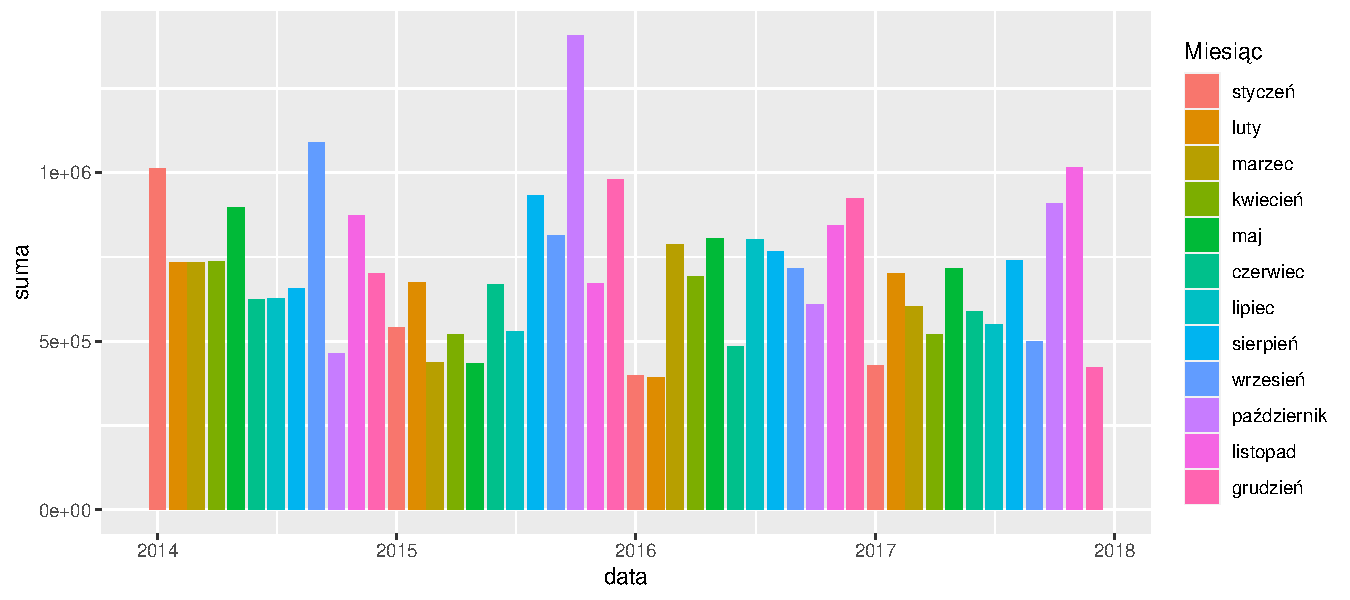
\includegraphics[width=\maxwidth]{figure/fig_zakup_pojazdu-1} 

}

\caption[Miesięczne wydatki na zakup pojazdów]{Miesięczne wydatki na zakup pojazdów}\label{fig:fig_zakup_pojazdu}
\end{figure}

\end{knitrout}

Wykres \ref{fig:fig_zakup_pojazdu} przedstawia miesięczne wydatki na zakup pojazdów. 
Największe wydatki warsztat miał w miesiącu wrzesień 2014. Były one w wysokości 1,17 mln. zł. 
Wydatki wielkości 1,07 mln. zł tyś. zł były drugimi najwyższymi i były \text{1,1} razy mniejsze od tych największych. Wystąpiły one w miesiącu styczeń 2014.
Najmniejsze wydatki warsztat zaobserwował w miesiącu lipiec 2017 i wyniosły one 372,3 tyś. zł. 
Drugie co do wielkości najniższe wydatki na zakup pojazdów wystąpiły miesiącu luty 2014, a wyniosły one 381,6 tyś. zł.
W każdym miesiącu działania warsztatu wydatki na zakup pojazdów wyniosły przynajmnej 400 tyś. zł.

\subsection{Analiza wydatków na zakup części}

Następnie zostało sprawdzone, jak wyglądają miesięczne wydatki na zakup części potrzebnych do napraw pojazdów.

\begin{knitrout}
\definecolor{shadecolor}{rgb}{0.969, 0.969, 0.969}\color{fgcolor}\begin{figure}[H]

{\centering 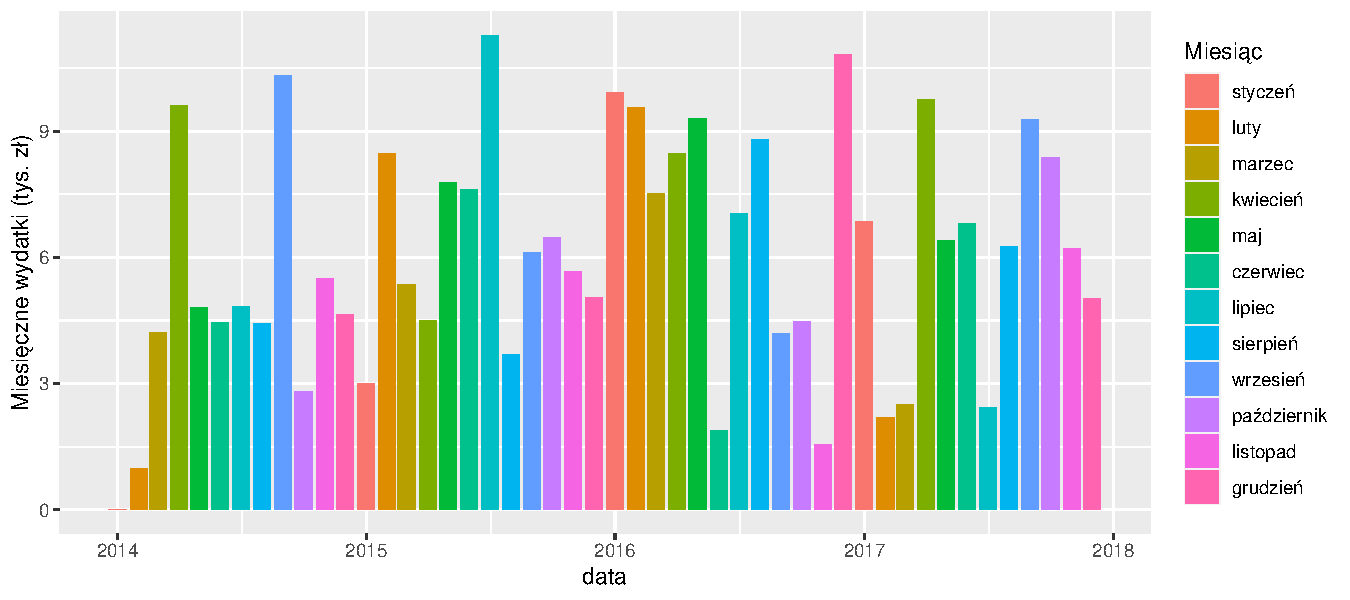
\includegraphics[width=\maxwidth]{figure/fig_zakup_czesci-1} 

}

\caption[Miesięczne wydatki na zakup części]{Miesięczne wydatki na zakup części}\label{fig:fig_zakup_czesci}
\end{figure}

\end{knitrout}

Wykres \ref{fig:fig_zakup_czesci} przedstawia miesięczne wydatki na zakup części do naprawy pojazdów.
Największe wydatki warsztat miał w miesiącu lipiec 2015 i wyniosły one 11,29 tyś. zł. 
Drugie najwyższe wydatkami były wielkości 10,82 tyś. zł i były \text{1,04} razy mniejsze od tych największych. Wystąpiły one w miesiącu grudzień 2016.
Najmniejsze wydatki na części zostały odnotowane w miesiącu styczeń 2014 i wyniosły 0 zł. 
Drugie najmniejsze wydatki wyniosły 973 zł. Wystąpił on w miesiącu luty 2014.
Ogólnie w każdym miesiącu działania warsztatu wydatki na zakup części wyniosły przynajmnej 0 zł.

\subsection{Analiza przychodów z usług warsztatu}

Chcielibyśmy sprawdzić, jak wyglądają miesięczne przychody (lub straty) wynikające z prowadzenia warsztatu. Przez przychód za pojedyńczą usługę uważamy różnicę ceny, którą zapłacił klient i kwoty zapłaconej za części. Przeanaliowane zostaną przychody z uwzględnieniem kosztu własnych napraw oraz bez nich.

\begin{knitrout}
\definecolor{shadecolor}{rgb}{0.969, 0.969, 0.969}\color{fgcolor}\begin{figure}[H]

{\centering 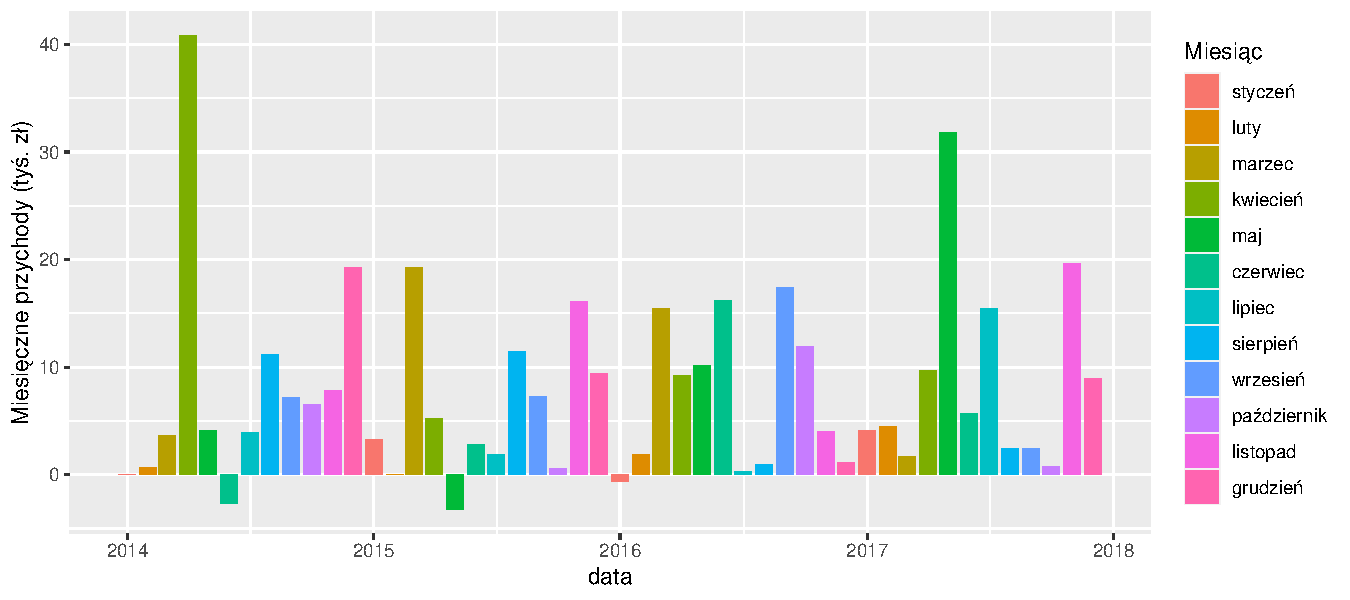
\includegraphics[width=\maxwidth]{figure/fig_uslugi-1} 

}

\caption[Miesięczny przychód wynikający z prowadzenia warsztatu z wliczonymi kosztami napraw własnych]{Miesięczny przychód wynikający z prowadzenia warsztatu z wliczonymi kosztami napraw własnych}\label{fig:fig_uslugi}
\end{figure}

\end{knitrout}

Na wykresie \ref{fig:fig_uslugi} przedstawiony jest miesięczny przychód wynikający z prowadzenia warsztatu. Zostały na nim uwzględnione koszty napraw własnych. 
Największy przychód był zaobserwowany w miesiącu styczeń 2016 i wyniósł on wtedy 27,19 tyś. zł.
Następny co do wielkości przychód wystąpił w miesiącu luty 2016, wyniósł on 22,94 tyś. zł. Jest on \text{1,18} razy mniejszy niż najwyższy przychód.
Najmniejszy przychód warsztat odnotował w miesiącu grudzień 2017, który wyniósł -2,28 tyś. zł. 
Drugi najmniejszy przychód wyniósł -335 zł i wystąpił w miesiącu listopad 2017.

\begin{knitrout}
\definecolor{shadecolor}{rgb}{0.969, 0.969, 0.969}\color{fgcolor}\begin{figure}[H]

{\centering 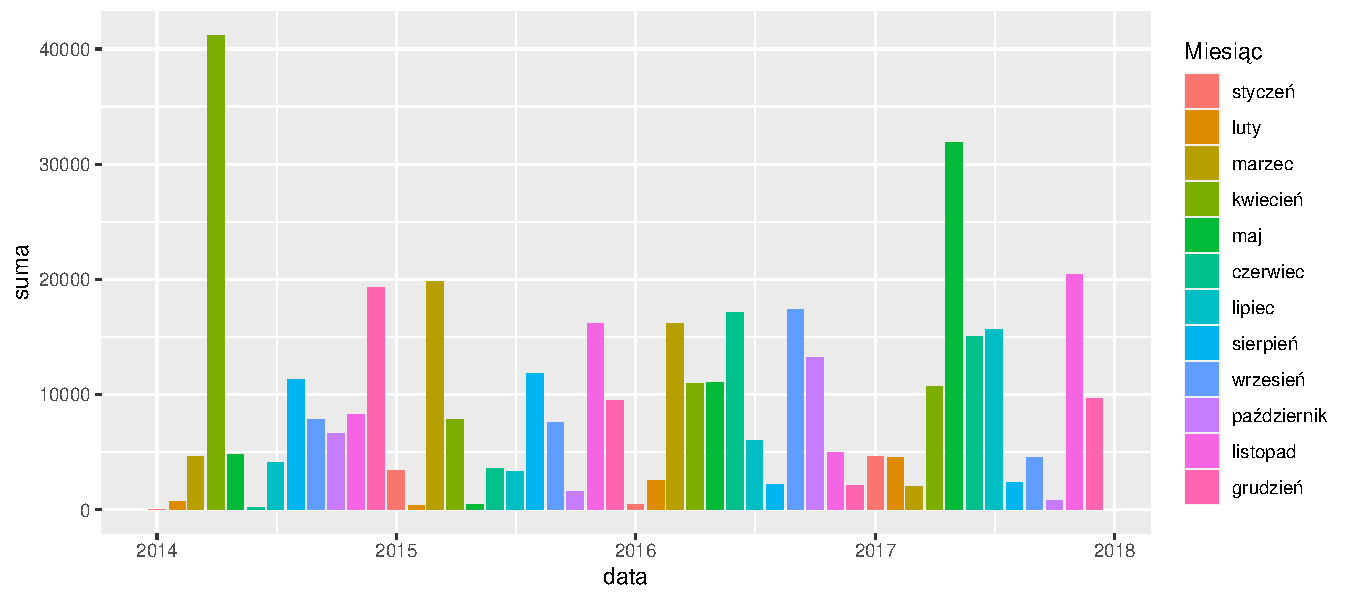
\includegraphics[width=\maxwidth]{figure/fig_uslugi2-1} 

}

\caption[Miesięczny przychód wynikający z prowadzenia warsztatu bez wliczonych kosztów napraw własnych]{Miesięczny przychód wynikający z prowadzenia warsztatu bez wliczonych kosztów napraw własnych}\label{fig:fig_uslugi2}
\end{figure}

\end{knitrout}

Na wykresie \ref{fig:fig_uslugi2} przedstawiony jest miesięczny przychód wynikający z prowadzenia warsztatu, ale tym razem bez uwzględnienia kosztów własnych. 
Największy przychód warsztat zaobserwował w miesiącu styczeń 2016, który wyniósł 27,19 tyś. zł.
Drugi zaś co do wielkości przychód wsytąpił w miesiącu luty 2016, wyniósł on 23,68 tyś. zł, czyli jest \text{1,15} razy mniejszy niż ten najwyższy zaobserwowany.
Najmniejszy przychód został odnotowany w miesiącu styczeń 2014 i wyniósł 0 zł. 
Drugi najmniejszy przychód wyniósł 947 zł. Wystąpił on w miesiącu grudzień 2017.

\subsection{Koszty wypłat dla pracowników}

Zostanie sprawdzone, jakie miesięczne koszty ponosi warsztat na wypłaty pensji dla pracowników.

%Zakładamy, że płaca w miesiącu to 160*płaca (przy zatrudnieniu/zwolnieniu pracownika patrze ile dni w miesiacu pracownik pracowal i robie ulamek, np. jak zatrudnili go 3 marca to dostaje round(płaca*160*29/31,2)) i podobnie ostatni to by byl round(płaca*160*3/31,2), wypłacamy pieniądze 1 dnia kolejnego miesiąca (np za styczeń wypłacamy 1 lutego)

\begin{knitrout}
\definecolor{shadecolor}{rgb}{0.969, 0.969, 0.969}\color{fgcolor}\begin{figure}[H]

{\centering 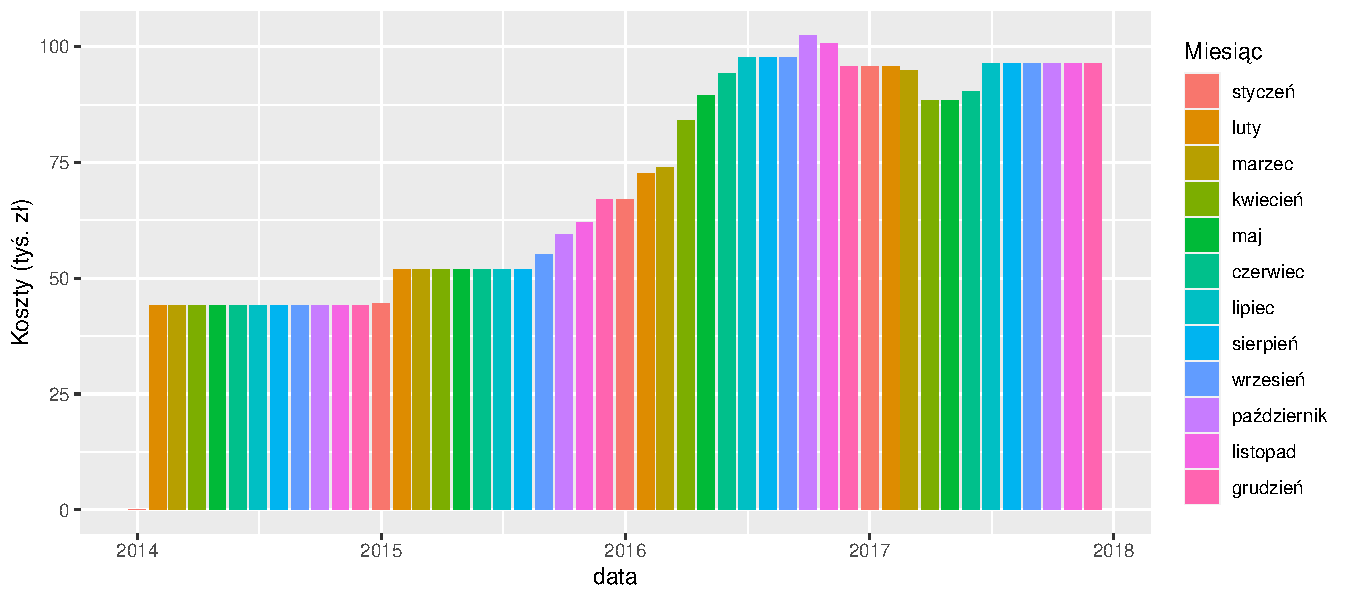
\includegraphics[width=\maxwidth]{figure/fig_pracownicy-1} 

}

\caption[Miesięczne koszty wynikające z wypłacania pensji pracownikom]{Miesięczne koszty wynikające z wypłacania pensji pracownikom}\label{fig:fig_pracownicy}
\end{figure}

\end{knitrout}

Wykres \ref{fig:fig_pracownicy} przedstawia miesięczne koszty wypłat pensji pracowników. Największy koszt warsztat odnotował w miesiącu grudzień 2017 i wyniósł on 103,28 tyś. zł. Zatem widać, że aktualnie warsztat ponosi największe koszty wynikające z wypłat dla pracowników. 
Natomiast najmniejsze koszty wystąpiły w miesiącu styczeń 2014. Wyniosły one 0 zł. Wynika to z tego, że jest to pierwszy miesiąc działania warsztatu, a pensje wypłacamy pracownikom pierwszego dnia następnego miesiąca.. Poza tym miesiącem najmniej wypłacono pracownikom w miesiącu luty 2014. Była to kwota 43,82 tyś. zł.

\subsection{Wpływy ze sprzedaży pojazdów}

Następnie zostaną sprawdzone miesięczne wpływy finansowe ze sprzedaży pojazdów, które zostały zakupione i w razie potrzeby naprawione przez warsztat. Pojazdy są sprzedawane na dwa sposoby: klient może zapłacić całą kwotę na raz lub spłacać w ratach.

\begin{knitrout}
\definecolor{shadecolor}{rgb}{0.969, 0.969, 0.969}\color{fgcolor}\begin{figure}[H]

{\centering 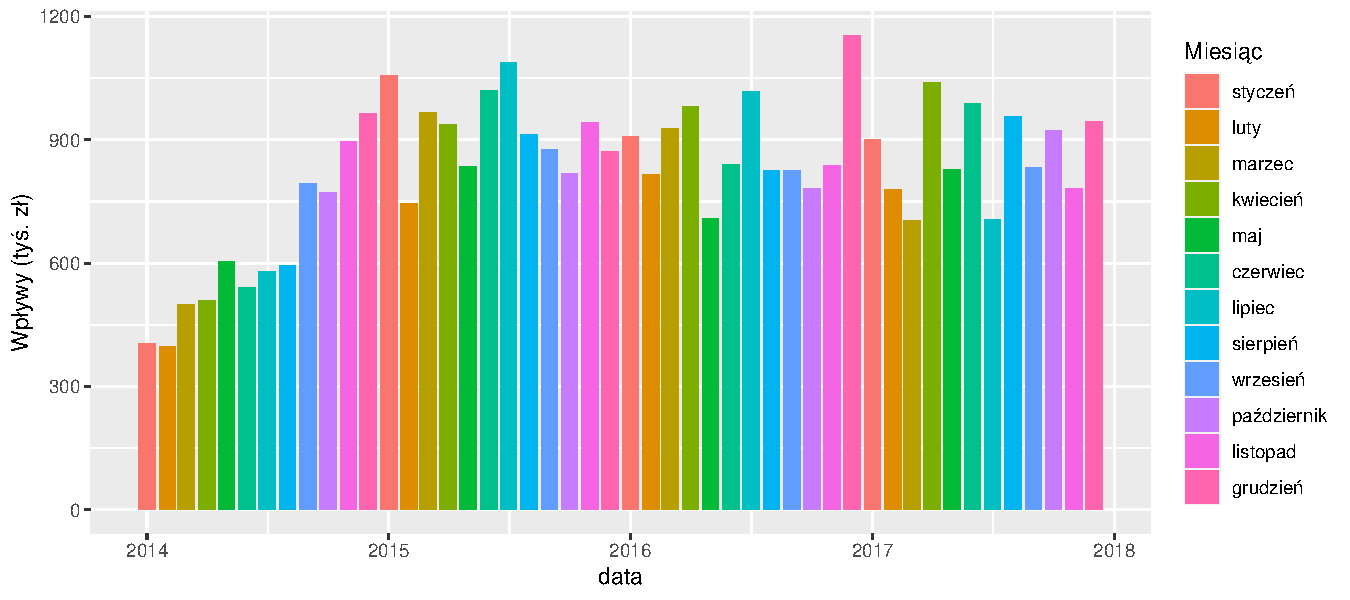
\includegraphics[width=\maxwidth]{figure/fig_samochody_wplywy-1} 

}

\caption[Miesięczne wpływy finansowe ze sprzedaży pojazdów]{Miesięczne wpływy finansowe ze sprzedaży pojazdów}\label{fig:fig_samochody_wplywy}
\end{figure}

\end{knitrout}

Na wykresie \ref{fig:fig_samochody_wplywy} przedstawione są wpływy finansowe ze sprzedaży pojazdów. 
Największe miesięczne wpływy warsztatu ze sprzedaży pojazdów wynosiły 1,15 mln. zł. Wystąpiły one w miesiącu grudzień 2016. 
Drugie co do wielkości wpływy (w wysokości 1,09 mln. zł) zostały odnotowane w miesiącu lipiec 2015. Są one \text{1,06} razy mniejsze niż te największe zaobserwowane.
Najmniejsze miesięczne wpływy wyniosły 0,39835494 zł, a wystąpiły one w miesiącu luty 2014.
Kolejnymi najmniejszymi są wpływy z miesiącu styczeń 2014. Są one wysokości 404,64 tyś. zł.


\subsection{Bilans miesięczny}

Teraz zostanie sprawdzony miesięczny bilans warsztatu. Zostaną sprawdzone miesięczne przychody warsztaty przez cały okres jego działania oraz comiesięczny stan środków finansowych firmy, gdyby warsztat zaczynał bez posiadania żadnych średków pienięznych.

\begin{knitrout}
\definecolor{shadecolor}{rgb}{0.969, 0.969, 0.969}\color{fgcolor}\begin{figure}[H]

{\centering 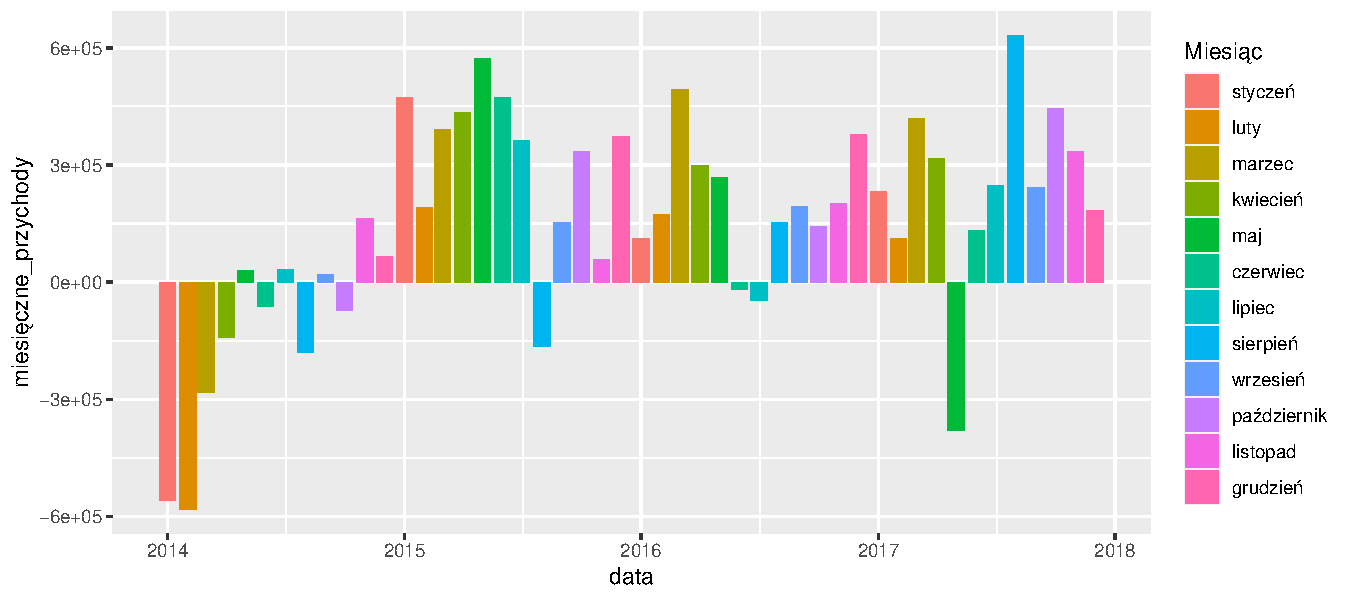
\includegraphics[width=\maxwidth]{figure/fig_bilans-1} 

}

\caption[Miesięczne przychody warsztatu]{Miesięczne przychody warsztatu}\label{fig:fig_bilans}
\end{figure}

\end{knitrout}

%złączenie: na miesiąc = naprawy(te z minusami, bo mają razem części) + sprzedaż pojazdu -zakup pojazdu - wypłaty (czy ja coś pominęłam?)

Wykres \ref{fig:fig_bilans} przedstawia miesięczne przychody firmy od początku jej działalności. 
Najwięcej warsztat zarobił (409,05 tyś. zł) w miesiącu grudzień 2017.
Natomiast najmniej w miesiącu styczeń 2014. Zyski wyniosły wtedy -662,16 tyś. zł. Przez pierwsze 5 miesięcy pracy warsztat nie przynosił żadnych zysków.

\begin{knitrout}
\definecolor{shadecolor}{rgb}{0.969, 0.969, 0.969}\color{fgcolor}\begin{figure}[H]

{\centering 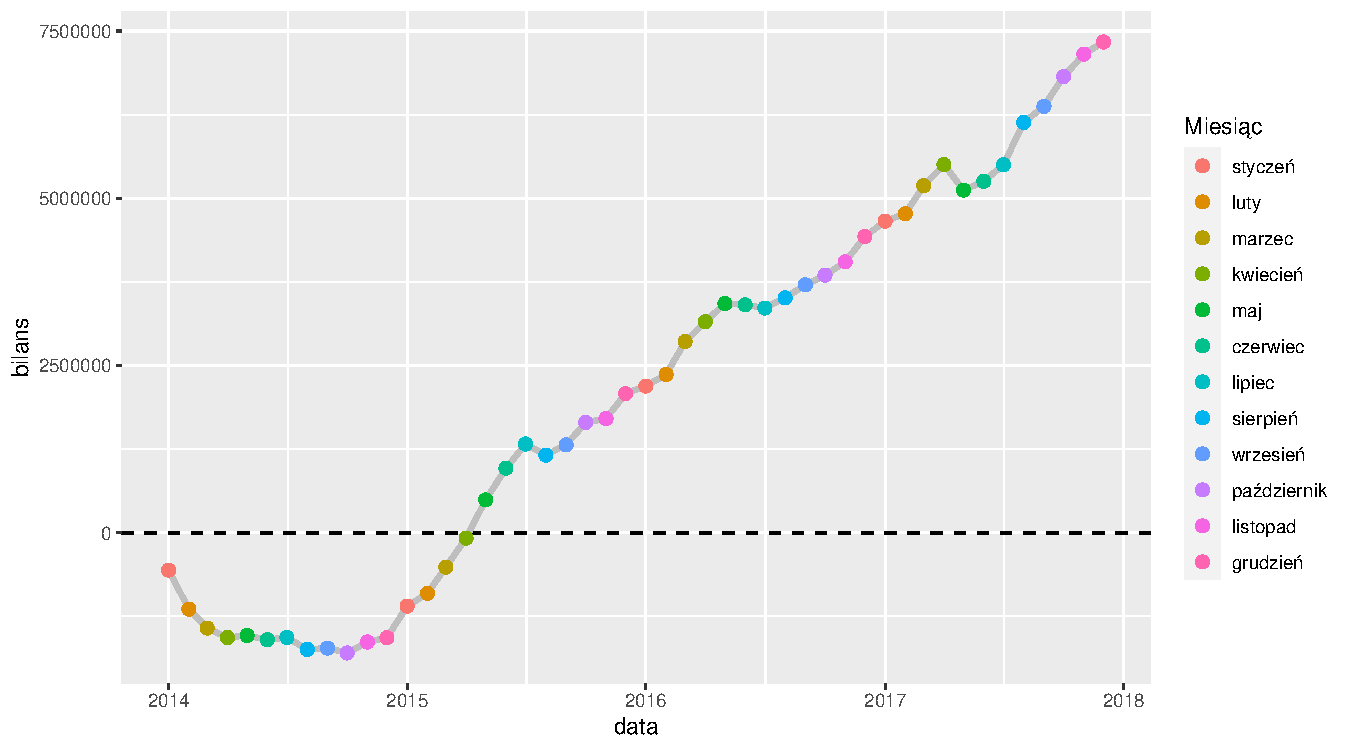
\includegraphics[width=\maxwidth]{figure/fig_bilans_suma-1} 

}

\caption[Miesięczny stan finansowy warsztatu, gdyby zaczynał działalność bez żadnych środków pieniężnych]{Miesięczny stan finansowy warsztatu, gdyby zaczynał działalność bez żadnych środków pieniężnych}\label{fig:fig_bilans_suma}
\end{figure}

\end{knitrout}

Wykres \ref{fig:fig_bilans_suma} przedstawia miesięczny stan finansowy warsztatu, gdyby zaczynał działalność bez środków pieniężnych. W pierwszym miesiącu działalności stan finansowy wyniósł -662,16 tyś. zł, natomiast aktualnie wynosi on 6,25 mln. zł. Przez pierwsze 17 miesięcy pracy warsztatu jego stan finansowy był ujemny.
Największą ilością pieniędzy warsztat operował w miesiącu grudzień 2017, było to 6,25 mln. zł.
Natomiast najmniejszą w miesiącu wrzesień 2014, a było to -1,54 mln. zł.

\section{Podsumowanie}
W tym raporcie przeanalizowano różne aspekty działalności warsztatu. Sprawdzano między innymi dane dotyczące sprzedaży i napraw pojazdów. Przeanalizowano także, jak wygląda grupa docelowa warsztatu, czyli jakie cechy mają nasi klienci. Poddano także analizie miesięczne przychody warsztatu i sprawdzono to, którzy pracownicy się najbardziej przyczynili do sukcesu firmy.




\end{document}
